% File tacl2018.tex
% Aug 3, 2018

% The English content of this file was modified from various *ACL instructions
% by Lillian Lee and Kristina Toutanova
%
% LaTeXery is all adapted from acl2018.sty.


% To check:
% - Submission must be in A4 format
% - min length 7 pages, max length 10 of CONTENT

% Example table:

% \begin{table}[t]
% \begin{center}
% \begin{tabular}{|l|rl|}
% \hline \bf Type of Text & \bf Size & \bf Style \\ \hline
% paper title & 15 pt & bold \\
% \iftaclfinal
% author names & 12 pt & bold \\
% author affiliation & 12 pt & \\
% \else
% \fi
% the word ``Abstract'' as header & 12 pt & bold \\
% abstract text & 10 pt & \\
% section titles & 12 pt & bold \\
% document text & 11 pt  &\\
% captions & 10 pt & \\
% %bibliography & 10 pt & \\
% footnotes & 9 pt & \\
% \hline
% \end{tabular}
% \end{center}
% \caption{\label{tab:font-table} Font requirements}
% \end{table}


\documentclass[11pt,a4paper]{article}
\usepackage[hyperref]{tacl2018} % use ``nohyperref'' to disable  hyperref
\usepackage{times,latexsym}
\usepackage{url}
\usepackage[T1]{fontenc}

\taclfinalfalse % For camera-ready, replace "\taclfinalfalse" with
% "\taclfinalcopy"

%%%%
%%%% Material in this block can be removed by TACL authors.
% It consists of things specific to generating TACL instructions
\usepackage{xspace,mfirstuc,tabulary}


% packages added by Marco and Michael
\usepackage{paralist} 
\usepackage{graphicx} 
\usepackage{multirow} 
\usepackage{enumitem}


\newcommand{\ex}[1]{{\sf #1}}

%
\iftaclfinal
\newcommand{\taclpaper}{camera-ready\xspace}
\newcommand{\taclpapers}{camera-readies\xspace}
\newcommand{\Taclpaper}{Camera-ready\xspace}
\newcommand{\Taclpapers}{Camera-readies\xspace}
\else
\newcommand{\taclpaper}{submission\xspace}
\newcommand{\taclpapers}{{\taclpaper}s\xspace}
\newcommand{\Taclpaper}{Submission\xspace}
\newcommand{\Taclpapers}{{\Taclpaper}s\xspace}
\fi

\newif\iftaclinstructions
\taclinstructionsfalse % AUTHORS: do NOT set this to true
\iftaclinstructions
\renewcommand{\confidential}{}
\renewcommand{\anonsubtext}{(No author info supplied here, for consistency with
TACL-submission anonymization requirements)}
\fi
%%%% End TACL-instructions-specific macro block
%%%%

\title{\emph{Tabula} nearly \emph{rasa:} Probing the linguistic knowledge of character-level neural language models trained on unsegmented text}


% The command \taclfinalfalse suppresses display of the contents of the
% \author{...} command in the generated pdf.
% Replacing that command with "\taclfinalcopy" reveals the author info in the
% generated pdf.
% See tacl2018.sty for other ways to set author info.
\author{
 Template Author\Thanks{The {\em actual} contributors to this instruction
 document and corresponding template file are given in Section
 \ref{sec:contributors}.} \\
 Template Affiliation/Address Line 1 \\
 Template Affiliation/Address Line 2 \\
 Template Affiliation/Address Line 2 \\
  {\sf template.email@sampledomain.com} \\
}

\date{}

\begin{document}
\maketitle
\begin{abstract}
As recurrent neural networks (RNNs) have recently reached striking performance levels in a variety of natural language processing tasks, there has been a revival of interest in whether these generic sequence processing devices are effectively capturing linguistic knowledge. Nearly all studies of this sort, however, initialize the RNNs with a vocabulary of known words, and feed them tokenized input during training. In the current work, we present an extensive, multi-lingual study of the linguistic knowledge discovered by RNNs trained at the character level on input data with word boundaries removed. Our networks, thus, face a tougher and more cognitively realistic task, having to discover all the levels of the linguistic hierarchy from scratch. Our results show that these ``near \emph{tabula rasa}'' RNNs are implicitly encoding a surprising amount of phonological, lexical, morphological, syntactic and semantic information, opening the doors to intriguing speculations about the degree of prior knowledge that is necessary for successful language learning.
\end{abstract}


\section{Introduction}
\label{sec:introduction}

Recurrent neural networks (RNNS), in particular their Long-Short-Term-Memory
variant \cite[LSTMs,][]{Hochreiter:Schmidhuber:1997} are the current workhorse
of natural language processing. These models, often pre-trained on the
simple \emph{language modeling} objective of predicting the next
symbol in raw natural text, form a crucial component of
state-of-the-art architectures for tasks such as machine translation,
natural language inference and text categorization
\cite{Goldberg:2017}.

RNNs are very general devices for sequence processing, assuming little
prior bias. Moreover, the simple prediction task they are trained on
in language modeling seems well-aligned with the core role prediction
plays in cognition \cite[e.g.,][]{Bar:2007,Clark:2016}. RNNS have thus
long attracted the attention of cognitive scientists and linguists
interested in language and processing, and their recent successes in
realistic large-scale tasks has strongly rekindled this interest
\cite[see, e.g.,][and references there]{Frank:etal:2013,Lau:etal:2017,Kirov:Cotterell:2018,McCoy:etal:2018,Pater:2018}.

Following the standard pre-processing pipeline for RNNs, these studies
assume that the input has been tokenized into words, and the latter
are pre-stored in the RNN vocabulary. This is a reasonable practical
approach, but it makes simulations less interesting from a language
learning point of view. First, discovering words is one of the major
challenges a learner faces, and by pre-encoding them in the RNN we are
facilitating its task in a very unnatural way (not even the staunchest
nativists would claim words to be part of our genetic code). Second,
assuming a unique tokenization into a finite number of discrete word
units is in any case problematic. The very notion of what counts as a
word in languages with a rich morphology is far from clear
\cite[e.g.,][]{Bickel:Zuniga:2017}, and, universally, mental lexicons
are probably organized into a not-necessarily-consistent hierarchy of
units at different levels: morphemes, words, compounds, constructions,
etc.~\cite[e.g.,][]{Goldberg:2005}.

Motivated by these considerations, we present here an extensive study
of RNNs trained on language modeling at the character level, or
\emph{character-level neural language models}
\cite[CNLMs,][]{Mikolov:etal:2011,Sutskever:etal:2011,Graves:2014}. Moreover,
the RNNs are trained on input where whitespace has been removed, so
that, like children learning a language, they don't have access to
major cues to wordhood.\footnote{We do not erase punctuation marks,
  reasoning that they have a similar function to prosodic cues in
  spoken language.} This setup is almost as \emph{tabula rasa} as it
goes: by taking unsegmented orthographic output (and assuming that, in
the alphabetic writing systems we work with, there is a reasonable
correspondance between letters and phonetic segments), we are only
assuming that a learner has figured out how to segment a continuous
speech stream into phonological units, an ability that children a few
months after birth \cite[e.g.,][]{Maye:etal:2002,Kuhl:2004}.

Our simulations involve phonological, morphological, syntactic and
semantic tests in English, German and Italian. Taken together, they
show that near-\emph{tabula rasa} CNLMs acquire an impressive spectrum
of linguistic knowledge at various levels.  This in turn suggests
that, given abundant input, a learning device that is only HERE

We study what linguistic knowledge CNMLs induce, simulating a
minimum-previous knowledge setup by training on corpora where white
space has been removed, thus without explicit cues to word
boundaries. We find that such models are discovering a remarkable
amount of linguistic information, at the phonotactic, lexical,
morphological, syntactic and semantic levels. This suggests that,
given abundant input, a learner can induce much linguistic knowledge
with almost no innate bias towards linguistic structures and,
intriguingly, without an explicit lexicon.




\section{Related work}
\label{sec:related}

\paragraph{Character-based neural language models} have received some attention in the last
decade because of their greater generality, and because, intuitively, they should be able to
use cues, such as morphological information, that word-based models
miss by design. Early studies such as \newcite{Mikolov:etal:2011},
\newcite{Sutskever:etal:2011} and \newcite{Graves:2014} established
that CNLMs (trained with whitespace where relevant) are in general not
as good at language modeling as their word-based counterparts, but lag
only slightly behind (note that character-level sentence prediction
involves a much larger search space than predicting at the word
level). \newcite{Sutskever:etal:2011} and \newcite{Graves:2014}
presented informal qualitative analyses showing that CNLMs are
learning basic linguistic properties of their input. The latter, who
trained LSTM-based models, also showed that they can keep track, to
some extent, of hierarchical structure. In particular, they are able
to correctly balance parentheses when generating text.

Our aim here is to understand to what extent CNLMs trained on
unsegmented input learn various linguistic constructs. This differs
from most recent work in the area, that has focused on \emph{character-aware}
architectures combining character- and word-level information to
develop state-of-the-art language models that are also effective in
morphologically rich languages \citep[see, e.g.,][and references
there]{Bojanowski:etal:2016,Kim:etal:2016,Gerz:etal:2018}. For
example, the influential model of Kim and colleagues performs
prediction at the word level, but uses a character-based convolutional
network to generate word representations. Other work focuses on
segmenting words into morphemes with character-level RNNs
\cite[e.g.,][]{Kann:etal:2016}, with emphasis on optimizing segmentation, as
opposed to our interest in probing what the network implicitly learned
about morphemes and other units through generic language
modeling.% Moreover, these networks are not exposed to constituents
% larger than words.


\paragraph{Probing linguistic knowledge of neural language models} Extensive work probes the linguistic properties of
word-based neural language models, as well as more complex
architectures such as sequence-to-sequence systems: see, e.g.,
\newcite{Li:etal:2016,Linzen:etal:2016,Shi:etal:2016,Adi:etal:2017,Belinkov:etal:2017,Hupkes:etal:2017,Kadar:etal:2017,Li:etal:2017,Conneau:etal:2018}.

Early work by Jeffrey Elman is close in spirit to ours. In particular,
\newcite{Elman:1990} reported phonotactics and word segmentation
experiments similar to ours, but using toy inputs. More recently,
\newcite{Sennrich:2017} explored the grammatical properties of
character- and subword-unit-level models that are used as components
of a machine translation system. He concluded that current
character-based decoders generalize better to unseen words, but
capture less grammatical knowledge than subword units. Still, his
character-based systems lagged only marginally behind the subword
architectures on grammatical tasks such as handling agreement and
negation. \newcite{Radford:etal:2017} also studied CNLMs with focus on understanding their
properties, but only in the domain of sentiment
analysis. \newcite{Godin:etal:2018} investigated the rules implicitly
used by supervised character-aware neural morphological segmentation
methods, finding in particular that the networks discover
linguistically sensible patterns. More closely related to our goals,
\newcite{Alishahi:etal:2017} probed the linguistic knowledge induced by
a neural network that receives unsegmented acoustic input. They used
however a considerably more complex architecture, trained on
multimodal data, and they focused on phonology. \newcite{Kementchedjhieva:Lopez:2018} recently presented a related study
probing the linguistic knowledge of plain character-level neural
language models. Their results are aligned with ours, as they show
that these models have knowledge of lexical and morphological
structure, and they capture morphosyntactic categories as well as
constraints on possible morpheme combinations. One of their most
intriguing results is that the model tracks morpheme boundaries in a
localist fashion through a single unit (we could not replicate the
result with our model).  They do not explore syntactic or semantic
knowledge, and they limit their study to English. Moreover, they
trained their models on input with whitespace, thus providing the
model with a major (and cognitively artificial) cue to word
boundaries.




\section{Experimental setup}
\label{sec:setup}

We extracted plain text from full English, German and Italian
Wikipedia dumps with
WikiExtractor.\footnote{\url{https://github.com/attardi/wikiextractor}}
We randomly extracted testing and validation sections consisting of
50,000 paragraphs each, and used the remainder for training. The
training sets contained 16M (German), 9M (Italian), and 41M (English)
paragraphs, corresponding to 819M, 463M and 2,333M words,
respectively. Order of paragraphs was shuffled for training; we did
not attempt to split by sentences. All characters were lower-cased.
For word segmentation and word-based language models, we tokenized and
tagged the corpora with
TreeTagger.\footnote{\url{http://www.cis.uni-muenchen.de/~schmid/tools/TreeTagger/}}

We used as vocabularies the most frequent characters from
each corpus, setting thresholds so as to ensure that all characters
representing phonemes were included, resulting in vocabularies of 60 (English), 73 (German), and 59 (Italian) characters.
We further constructed \emph{word-level neural language models} (WordNLMs); 
their vocabulary included the most frequent 50,000 words per corpus.

We trained RNN and LSTM CNLMs; we will refer to them simply as
\emph{RNN} and \emph{LSTM}, respectively. We used LSTM cells for
WordNLMs.  For each model/language, we applied random
hyperparameter search.  We terminated training after 72 hours; none of
the models had overfitted, as measured by performance on the
validation set, used for model selection.\footnote{The selected
  hyperparameters are reported in supplementary material to be made
  available upon publication.}

Language modeling performance on the test partitions is shown in
Table~\ref{tab:lm-results}. Recall that we removed whitespace, which
is both easy to predict, and aiding prediction of other
characters. Consequently, the fact that our character-level models are
below the state of the art is expected.\footnote{Training our models
  with whitespace, without further hyperparameter tuning, resulted in
  BPCs of 1.32 (English), 1.28 (German), and 1.24 (Italian).}
For example, the best model of \newcite{merity2018analysis} achieved
1.23 English BPC on a Wikipedia-derived dataset. % (Hutter 2018). %, and 1.175 on a version of PTBenglish 0.85 german 0.9, italian 0.82
On EuroParl data, \newcite{cotterell2018all} report 0.85 for English,
0.90 for German, and 0.82 for Italian. Still, our English BPC is
comparable to that reported by \newcite{Graves:2014} for his static
character-level LSTM trained on space-delimited Wikipedia data,
suggesting that we are achieving reasonable performance.
%\footnote{Training our models on text with whitespace, without further hyperparameter tuning to adjust to that setting, resulted in cross-entropies of 0.91, 1.32 BPC (English), 0.89, 1.28 BPC (German), and 0.86, 1.24 BPC (Italian).}
The perplexity of the word-level model might not be comparable to
that of highly-optimized state-of-the-art architectures, but it is at the
expected level for a well-tuned vanilla LSTM language model. For
example, \newcite{Gulordava:etal:2018} report 51.9 and 44.9 perplexities respectively in English and Italian for
their best LSTMs trained on Wikipedia data with the same vocabulary
size as ours.
%=======
%Performance on the test partitions is shown in Table~\ref{tab:lm-results}.
%Direct comparison with the state-of-the-art in character-based language modeling is hindered by the fact that we train on text without whitespace.
%The best models of \cite{merity2018analysis} achieved 1.232 BPC on enwiki8 \cite{hutter2018}, a dataset also derived from English Wikipedia. % (Hutter 2018). %, and 1.175 on a version of PTBenglish 0.85 german 0.9, italian 0.82
%On Europarl data, \cite{cotterell2018all} report 0.85 for English, 0.9 for German, and 0.82 for Italian. 
%Our BPC values are higher, but this is expected given that we do not provide whitespace to the model: Whitespace is both relatively easy to predict, and it makes predicting other characters easier.\footnote{Refitting our models to data with whitespace, without retuning hyperparameters, yields ....}
%>>>>>>> 86b9fd533dc18bab83a010158126d7366aae3681

\begin{table}[t]
  \begin{small}
  \begin{center}
    \begin{tabular}{l|l|l|l}
      \multicolumn{1}{c|}{}&\emph{LSTM}&\emph{RNN}&\emph{WordNLM}\\
      \hline
	    English & 1.62 & 2.08 & 48.99  \\
	    German &  1.51 & 1.83 & 37.96   \\
	    Italian & 1.47 & 1.97 & 42.02  \\
    \end{tabular}
  \end{center}
  \end{small}
  \caption{\label{tab:lm-results} Performance of language models. For CNLMs, we report bits-per-character (BPC). For WordNLMs, we report perplexity.}
\end{table}

%\begin{table}[t]
%  \begin{center}
%    \begin{tabular}{l|l|l|l|l}
%      \multicolumn{1}{c}{}&\emph{LSTM}&\emph{RNN}&\emph{Word LSTM}\\
%      \hline
%	    English & 1.12 / 1.62 & 1.44 / 2.08 & 3.89 / 48.99  \\
%	    German &  1.05 / 1.51 & 1.27 / 1.83 & 3.63 / 37.96   \\
%	    Italian & 1.02 / 1.47 & 1.37 / 1.97 & 3.85 / 42.02  \\
%    \end{tabular}
%  \end{center}
%  \caption{\label{tab:lm-results} Performance of language models. For CNLMs, we report cross-entropy and bits-per-character (BPC). For word-based models, we report cross-entropy and perplexity.}
%\end{table}









\section{Experiments}
\label{sec:experiments}


\subsection{Discovering phonological classes}

We conducted agglomerative clustering of character embeddings in the output layer.
We found that, in all three languages, the highest-level clusters separated characters into consonants, vowels, numerals, punctuation, and various non-phonetic or rare characters.
In Figure~\ref{fig:char-clustering}, we show a clustering of German character embeddings restricted to alphabetic characters.
The top-level split partitions characters into vowels and consonants.
%Parts of the finer clustering can be phonologically motivated, e.g., the liquids r, l form a cluster
Consonant and vowel clusters each can, to a large extent, be phonologically motivated, though not along a single consistent dimensions:
(TODO describe)
%
%Within the vowel cluster: in German, vowels and their fronted umlauts together (understandable as a consequence of morphological alternations), also e/i 
%
%Clustering of consonants can partly be motivated phonologically, though not along a single consistent dimensions:
%In German, there are clusters sharing place of articulation (p/f, b/v/w, c/k/q). %, and the liquids (n/l/r) form a class 
%

\begin{figure}
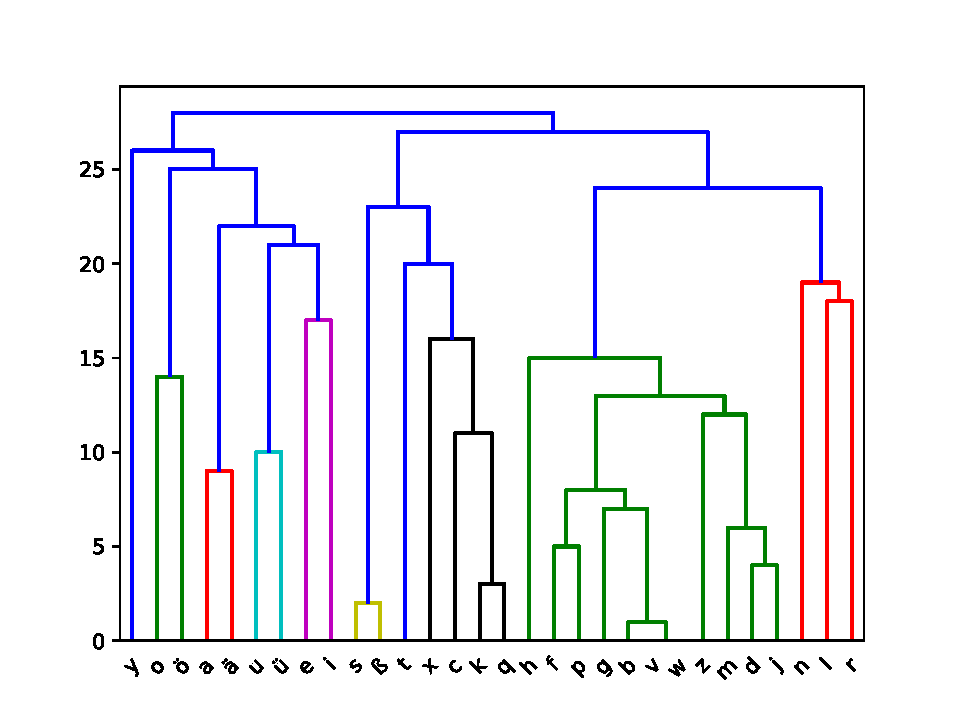
\includegraphics[width=0.50\textwidth]{figures/char-emb-clustering-output_output-phonetic-wiki-german-nospaces-bptt-910515909.pdf}
%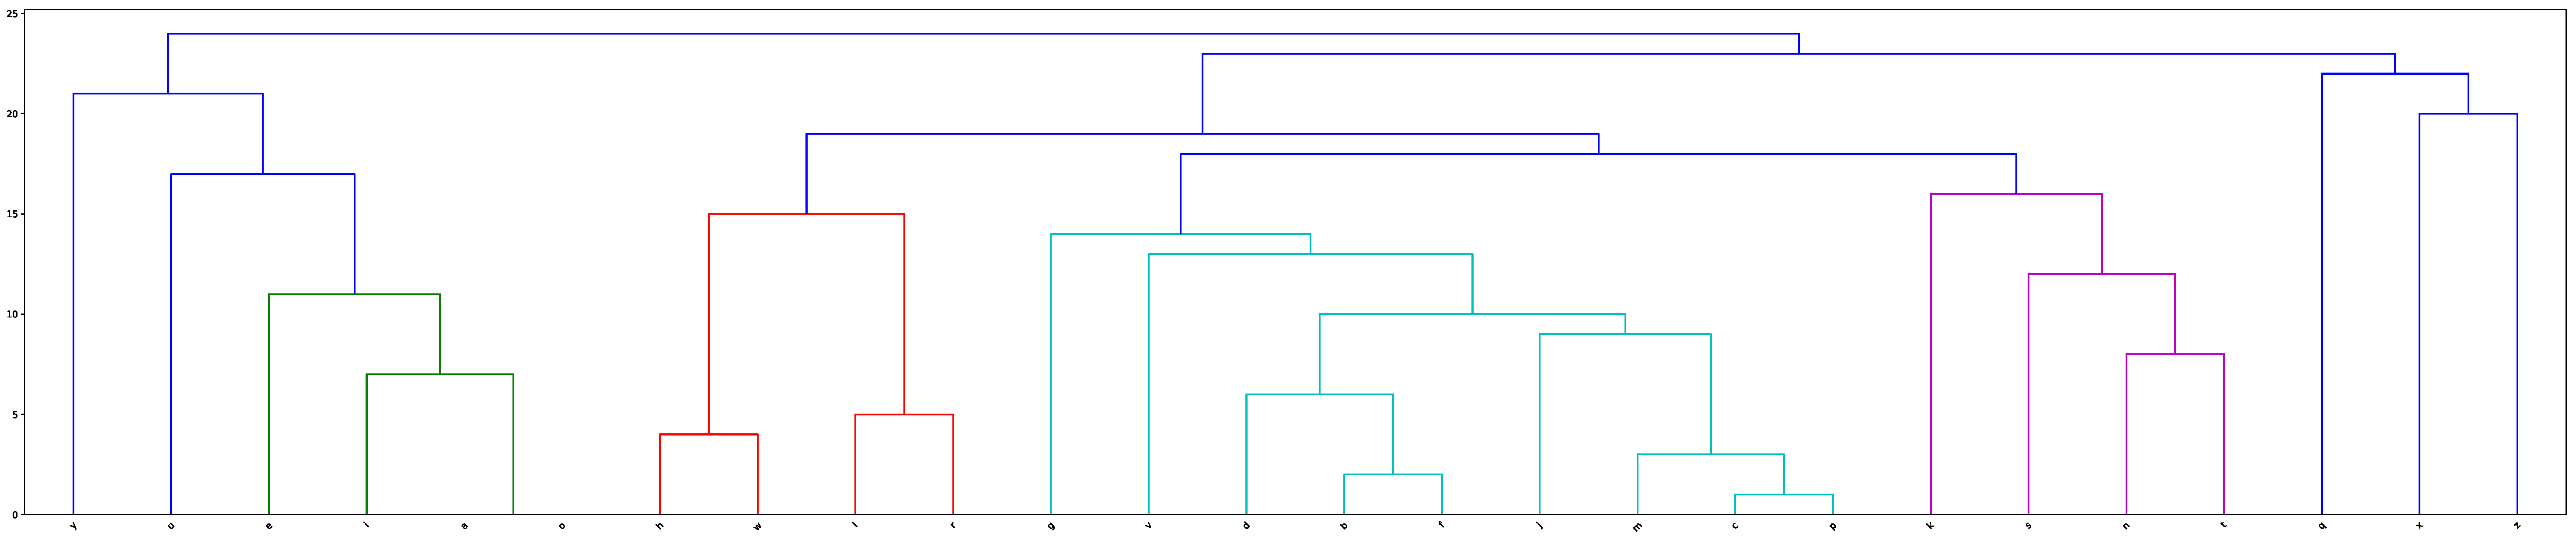
\includegraphics[width=0.48\textwidth]{figures/char-emb-clustering-output_output-phonetic-wiki-english-nospaces-bptt-282506230.pdf}
	%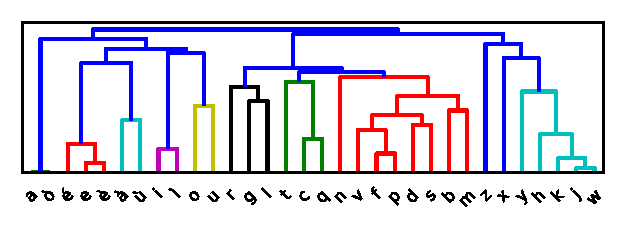
\includegraphics[width=0.48\textwidth]{figures/char-emb-clustering-output_output-phonetic-wiki-italian-nospaces-bptt-855947412.pdf}
\caption{Clustering of German character embeddings (alphabetic characters only)}\label{fig:char-clustering}
\end{figure}




\subsection{Discovering phonotactic constraints}
\label{sec:phonotactics}

Next, we study the CNLM's understanding of phonotactic constraints.
We focus on German and Italian, as they have reasonably transparent orthographies.
We construct pairs of letter bigrams (corresponding to phoneme
bigrams) beginning with the same letter, such that one is
phonotactically acceptable in the language and the other isn't, but
the independent unigram probability of the unacceptable bigram is
higher than that of the acceptable one. E.g., ``\emph{br}'' is
an acceptable Italian sequence and ``\emph{bt}'' isn't, although
\emph{``t''} is more frequent than \emph{``r''}.
For each such pair, we re-train the CNLM on a version of
the training partition from which all sequences containing either bigram have been removed.
We then look at
the likelihood the model assigns to both sequences. If the model systematically
assigns a larger probability to correct sequences, this provides evidence that it
implicitly possesses a notion of phonological categories such as
stops and sonorants, which allows it to correctly generalize from
attested (e.g., ``\emph{tr}'') sequences to unattested ones
(\emph{``br''}).

%We constructed bigram pairs where the second element was a vowel or a sonorant in the valid bigram, randomly choosing among possible vowels or sonorants if there were several.

In both languages, we constructed two groups of bigrams:
In one, the valid bigram had a vowel following a consonant; in the other, a consonant was followed by a sonorant.
In the invalid bigram, the consonant was followed by a stop or nasal.
For each onset consonant and each of the two types, we considered valid vowels or sonorants satisfying the constraint on unigram frequencies, and randomly selected one if there were several.

Results are shown in \ref{tab:phonotactics-results}.
The LSTM assigns higher probability to the valid bigrams in all but two cases.
The RNN, on the other hand, prefers the invalid bigrams, presumably because they have higher unigram probability.

This confirms that the LSTM CNLM has learnt a notion of phonological categories such as vowels and consonants, and phonotactic generalizations about them.
Note that the model makes these phonotactic generalizations entirely on the basis of distributional evidence, with no aid from perceptual or acrticulatory cues.



\begin{table}[t]
  \begin{center}
	  \begin{tabular}{p{0.2cm}p{0.2cm}|p{0.6cm}p{0.6cm}||p{0.2cm}p{0.2cm}|p{0.99cm}p{0.8cm}}
	    \multicolumn{4}{c||}{\emph{German}}   &       \multicolumn{4}{c}{\emph{Italian}}\\      \hline
	    \multicolumn{2}{c}{\emph{}}&\emph{LSTM}&\emph{RNN} & \multicolumn{2}{c}{\emph{}}&  \emph{LSTM}&\emph{RNN}\\      \hline
                     bu &  bt &  \textbf{ 4.6} &  0.22             &  bu & bd & \textbf{ 1.001} & 6e-5 \\            
                     do &  dd &  \textbf{ 1.9} &  0.05             &  du & dt & \textbf{ 1.3} & 0.008 \\             
                     fu &  ft &  \textbf{ 6.5} &  0.03             &  fu & ft & \textbf{ 30.5} & 0.01 \\             
                     po &  pt &  \textbf{ 6.4} &  0.10             &  pu & pt & \textbf{ 6.8} & 0.008 \\             
                     tu &  tt &  \textbf{ 5.4} &  0.02             &  tu & td &  0.2 & 3e-5 \\                       
		     zu &  zt &  \textbf{ 2.4} &  0.17             &  vu & vd & \textbf{ 2.0} & 2e-5 \\              \cline{1-4}
                     bl &  bd &   0.8          & 0.18              &  zu & zt & \textbf{ 55.7} & 0.01 \\              \cline{5-8} 
                     fl &  fd &  \textbf{ 2.1} & 0.82              &  br & bt & \textbf{ 1.001}  &  0.006           \\ 
                     fr &  fn &  \textbf{ 2.7} & 0.10              &  dr & dt & \textbf{ 2.5} & 0.4 \\               
                     kl &  kt &  \textbf{ 3.8} & 0.10              &  fr & ft & \textbf{ 2.9} & 0.001 \\             
                     pl &  pt &  \textbf{ 2.5} & 0.86              &  pr & pt & \textbf{ 5.0} & 0.008 \\              \hline
	    \multicolumn{2}{c|}{AM}      & \textbf{3.6} & 0.24     & 	    \multicolumn{2}{c|}{AM}   & \textbf{10.7}  & 0.041          \\
	    \multicolumn{2}{c|}{GM} & \textbf{3.0} & 0.13          & 	    \multicolumn{2}{c|}{GM}   & \textbf{3.2} & 0.0021           \\
      \hline
    \end{tabular}
  \end{center}
	\caption{\label{tab:phonotactics-results} Likelihood ratio between acceptable and unacceptable bigrams, with arithmetic (AM) and geometric (GM) means. Values $>1$ in bold.}
\end{table}

\subsection{Word segmentation}
\label{sec:segmentation}



Does the model develop an implicit notion of word?
Early work on word segmentation suggests that high uncertainty about the next character \cite{cohen-algorithm-2001, feng-accessor-2004},  low transition probabilities \cite{harris-distributional-1954, saffran-word-1996} and low mutual information \cite{sun-chinese-1998} serve as statistical cues to word segmentation.
In Figure~\ref{fig:syntax-depth}, we plot (1) entropy of the predicted distribution over the net character around word boundaries, compared to other positions, and (2) the pointwise mutual information (PMI) between left and right contexts, computed by subtracting the unconditional likelihood of the next 20 characters from their likelihood conditioned on the prior context, both computed by the CNLM on a section of the German training set.
In accordance with prior work, higher entropy and lower PMI correlate with boundaries.


\begin{figure}
	\begin{center}
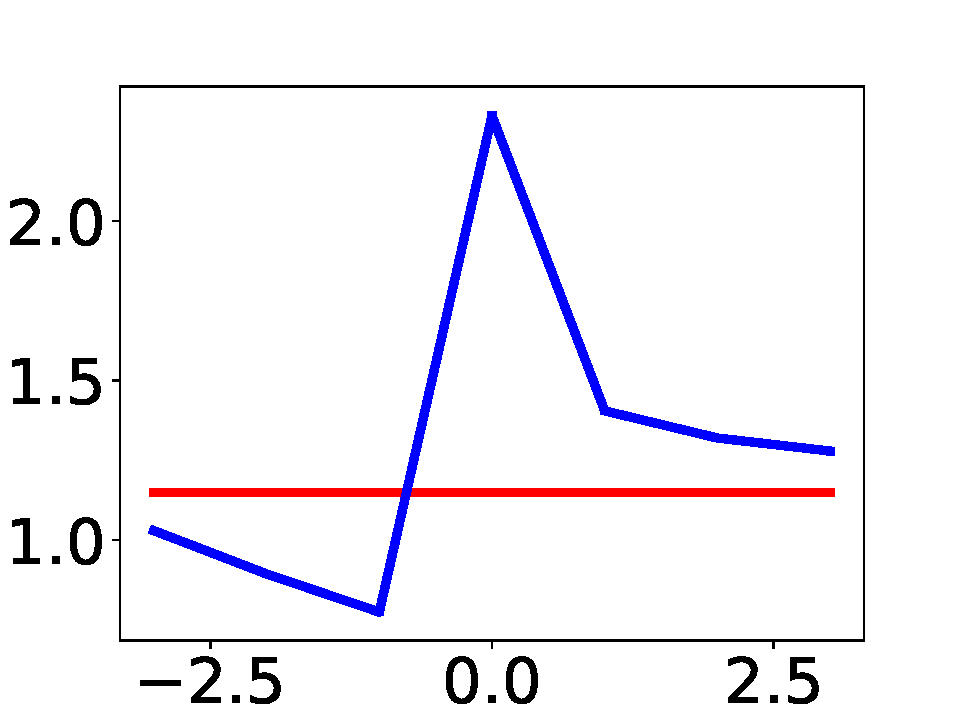
\includegraphics[width=0.22\textwidth]{figures/segmentation-profile-flattened-entropies-english-ci.pdf}
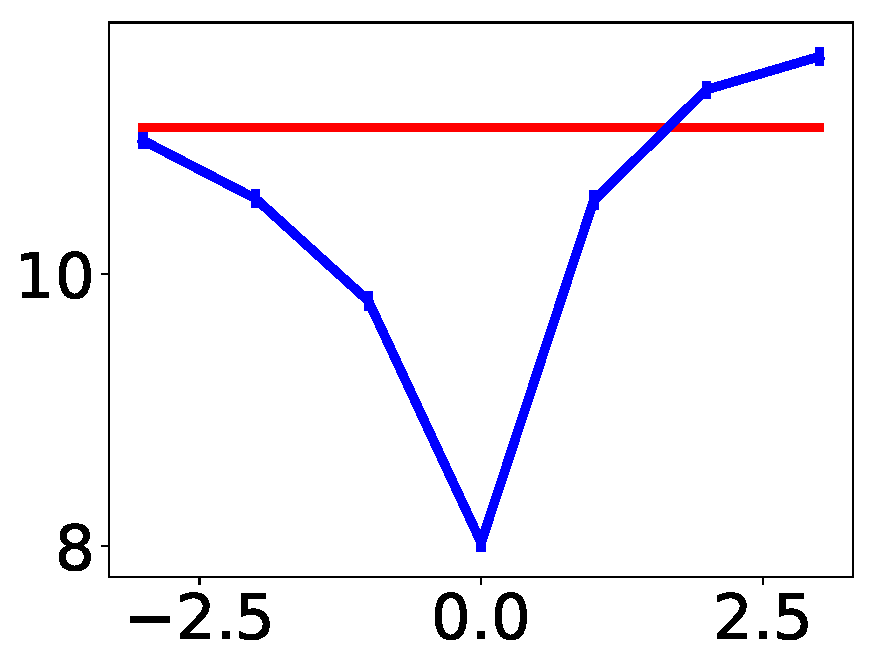
\includegraphics[width=0.22\textwidth]{figures/segmentation-profile-flattened-pmis-english-ci.pdf}
	\end{center}
	\caption{Entropy over the next character (left) and PMI between left and right contexts (right) around word boundaries (blue); the x-axis indicates position relative to a word boundary. The red line indicates the overall average of the quantity. Error bars indicate (almost imperceptible) bootstrapped 95 \% confidence intervals.
}\label{fig:boundaries-entropy}
\end{figure}


How reliable are these statistical cues, when computed by the CNLM?
We constructed a logistic regression predicting whether a character was the first one of a word or not, based on the following predictors:
(1) \emph{log-probability} of the character given prior context, (2) \emph{entropy} of the distribution over the character given prior context, (3) \emph{pmi of left and right contexts}, that is, the total likelihood of the next 20 characters, minus the unconditional likelihood estimated by starting the CNLM at the current position.
%The rationale of (3) is that it measures the pointwise mutual information, and thus the statistical association, between the subsequent characters and the prior context, which we hypothesize will be higher inside words.
%It is also the transition probability for the next characters
%(3) can also be interpreted as the result of normalizi transition probability
We collected these quantities for each position and for the preceding and following three characters.
%In total, the classifier has 21 coefficients.
We also conducted the same experiment with a character-level 8-gram model estimated on the training set, closer to the setup of earlier non-neural work.


\begin{table*}[t]
  \begin{center}
    \begin{tabular}{l|l|l|l|l}
      \multicolumn{1}{c}{}&\emph{LSTM}&\emph{RNN}&\emph{8-grams}\\
      \hline
      English & 65.83/60.37/62.98 &   63.26/59.81/61.49 & 55.73/51.0/53.26    \\ % \ldots{}/\ldots{}/\ldots & \ldots{}/\ldots{}/\ldots & \ldots{}/\ldots{}/\ldots &\ldots{}/\ldots{}/\ldots\\
      German &  57.012/52.505/54.67 &  53.2/49.26/51.15 & 42.89/36.28/39.31   \\ %   \ldots{}/\ldots{}/\ldots & \ldots{}/\ldots{}/\ldots & \ldots{}/\ldots{}/\ldots &\ldots{}/\ldots{}/\ldots\\
      Italian &  63.59/56.95/60.09 & 62.47/57.5/59.89  & 48.41/39.62/43.57    \\ % \ldots{}/\ldots{}/\ldots & \ldots{}/\ldots{}/\ldots & \ldots{}/\ldots{}/\ldots &\ldots{}/\ldots{}/\ldots\\
    \end{tabular}
  \end{center}
  \caption{\label{tab:segmentation-results} Precision recall, and F1 on word segmentation.}
\end{table*}

%PMI alone 
%P 30.56 R 20.61 F 24.61 German
%P 32.19 R 20.89 F 25.34 Italian
%P 39.37 R 29.45 F 33.69 English
%Surprisal alone
%P 28.04 R 18.64 F 22.4 German
%P 28.76 R 18.31 F 22.38 Italian
%P 33.65 R 24.1 F 28.08 English
%Entropy alone
%P 50.88 R 45.57 F 48.08 German
%P 58.44 R 52.09 F 55.08 Italian
%P 59.85 R 53.75 F 56.63 English


For each language model and language, we compute how many of the extracted tokens were correct (precision) and how many of the actual tokens were found by the classifier (recall), together with F1.
The goal of this experiment is not to construct a new word segmentation system, but to evaluate how strongly the CNLM's probabilities are indicative of word boundaries.

Results are shown in Figure~\ref{tab:segmentation-results}, showing that the CNLM-based classifiers robustly segment more than half of the tokens correctly, and do considerably better than the character 8-gram model.
Ablation shows that entropy is most predictive, reaching an F1 of 56.63 (English), 48.08 (German), 55.08 (Italian) alone.
Surprisal reaches 28.08 (English), 22.4 (German), 22.38 (Italian); PMI reaches 33.69 (English), 24.61 (German), 25.34 (Italian).
%Setting N to other values shows that larger values of N increase performance (N =10: 62.45, N=20: 63.24).

How does the LSTM CNLM compare to unsupervised word segmentation models?
We compare to the Bayesian bigram model of \cite{goldwater-bayesian-2009}, an elegant model using a hierarchical Dirichlet process.
Running Bayesian methods on the Wikipedia dumps is computationally infeasible; thus we also created a CNLM on the Brent corpus \cite{brent-efficient-1999} of child-directed speech.
We used 90 \% to train our language model, 5 \% to fit the logistic regression, and 5 \% to evaluate word segmentation.
(This compares with the Bayesian models that train and evaluate on the full dataset, but incorporate no word boundary information in their training signal).

\begin{table*}[t]
  \begin{center}
    \begin{tabular}{ll|l|l|l|l}
      \multicolumn{2}{c|}{}&Tokens & Lexical & Boundaries\\      \hline
	    \multirow{4}{*}{CNLM} & Full model & 0.75/0.76/0.75 & 0.41/0.61/0.49 & 0.91/0.90/0.90 \\
	    &     log-probability & 0.510/0.453/0.480 & 0.488/0.195/0.279 & 0.805/0.716/0.758 \\
	    &     entropy & 0.504/0.533/0.518 & 0.520/0.211/0.300 & 0.790/0.747/0.768\\
	    &     PMI & 0.708/0.729/0.718 & 0.576/0.346/0.432 &0.899/0.873/0.886  \\ \hline
	    \multicolumn{2}{c|}{\citet{goldwater-bayesian-2009}} & 0.752/0.696/0.723 & 0.635/0.552/0.591 & 0.903/0.808/0.852
    \end{tabular}
  \end{center}
	\caption{\label{tab:segmentation-results-brent} Word segmentation results on the Brent corpus for our model, for the three individual predictors, and the Bayesian model of \cite{goldwater-bayesian-2009}. Following \cite{goldwater-bayesian-2009}, we evaluate on the level of tokens, the lexicon of induced word types, and boundaries.}
\end{table*}

Results in Table~\ref{tab:segmentation-results-brent} show that the performance is broadly comparable to that of a sophisticated Bayesian segmentation method.
This suggests that statistical properties as modeled by the CNLM provide reliable cues to word boundaries.\footnote{We also created a logistic regression on hidden states, obtaining accuracy over 90 \% in classifying word boundaries on unseen words, outperforming an n-gram-count baseline. This suggests that the model internally tracks word boundaries.}
In contrast to the Wikipedia experiments, PMI emerges as the most important predictor on this dataset.

Unlike our method, the Bayesian method is fully unsupervised, but it has a built-in bias towards a discrete lexicon with a power-law frequency distribution.
Note that, unlike supervised word segmentation methods, our classifier does not have access to the character strings directly; instead, it evaluates how strongly quantities computed by the CNLM \emph{correlate} with word boundaries.



Looking at the main errors made by our English CNLM is instructive. We
consider first the 30 most common undersegmentations in the test set
(that is, cases in which the model failed to split two or more
words). About half (16) of them are common function word sequences
that could indeed easily be re-analyzed as single words (e.g.,
\emph{more than}, \emph{as well as}, \emph{such as}). Of the remaining
cases, 8 follow the \emph{N of} pattern, where \emph{N} is a
(typically relational) noun commonly occurring in this construction
(\emph{member of}, \emph{end of}, \emph{part of}\ldots). There are 3
fixed multi-word expressions (\emph{New York}, \emph{United States}
and \emph{high school}). Finally, it's reasonable to treat \emph{based
  on}, \emph{known as} and \emph{according to} as lexicalized
connectives, especially in the Wikipedia text the model was trained
upon.

The picture is a bit murkier but still fairly linguistically grounded
for the 30 most common oversegmentation errors (that is, the character
fragments that are wrongly segmented from inside the largest number of
distinct words).\footnote{We ignore here single-letter segmentations,
  that would otherwise account for one third of the most-frequent
  set.}  More than half (17) are common affixes (prefixes such as
\emph{re} and \emph{de} or suffixes such as \emph{ing} and
\emph{ly}). The remaining cases include 3 strings identical to frequent
function words wrongly carved out of longer words (\emph{the},
\emph{to} and \emph{on}, although the model might be treating the
latter as a pseudo-suffix in forms such as \emph{Peterson} and
\emph{Creighton}). Further, the strings \emph{land} and \emph{man} are not
unreasonably segmented out of compounds. It's hard, on the other hand,
to find a linguistically sound motivation for the 8 remaining top
oversegmentations (\emph{la, le, ma, na, ra, ro, se, ta}).

We hypothesized that similar statistical correlates exist for hierarchical syntactic structure.
We created constituency trees for the German validation set using the Berkeley Parser~\ref{petrov2007improved}.
For each character in the data, we counted its hierarchical distance from the preceding character, operationalized as the number of intervening closing and opening brackets.
This number is zero if and only if both characters belong to the same word.

Figure~\ref{fig:syntax-depth} plots PMI by hierarchical distance, for all distances for which at least 1000 datapoints occurred in the dataset.
The plot shows that longer hierarchical distance between neighboring characters corresponds to lower average MI, generalizing the finding for word boundaries.
This illustrates how it is useful for segmentation knowledge to be implicit, as the model ``knows'' about different kinds of boundaries in a continuous manner.

\begin{figure}
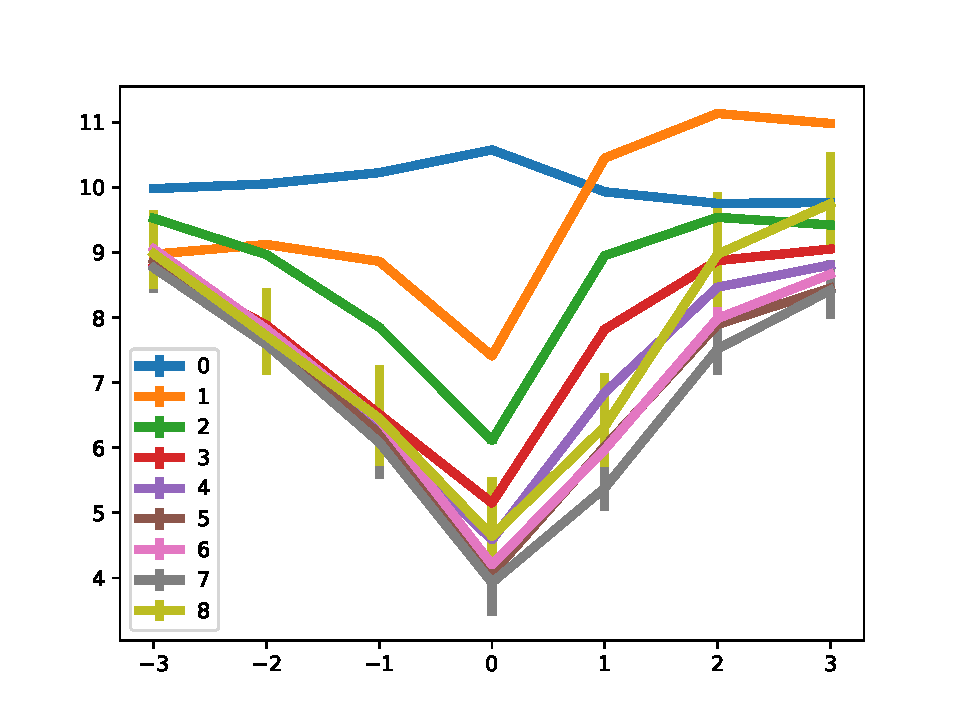
\includegraphics[width=0.48\textwidth]{figures/segmentation-profile-pmis-german-all-heights-ci.pdf}
\caption{PMI between left and right contexts, estimated by the CNLM, by syntactic hierarchical distance between subsequent characters, and bootstrapped 95 \% confidence intervals.}\label{fig:syntax-depth}
\end{figure}



%687112
%73757
%46716
%22847
%7896
%2587
%827
%234
%80




\subsection{Discovering morphological categories}
\label{sec:categories}

Does the CNLM discover morphological categories?
Note that these are lexical
properties, probed in a model that has no explicit notion of word.
We again focus on German and Italian given massive morphosyntactic ambiguity
and impoverished morphology of English.

\paragraph{Word classes (nouns vs.~verbs)}

Does the model implicitly encode word classes?
We sampled 500 verbs and 500 nouns from the training set, each with the requirement that they end in -\emph{en} (German) or -\emph{re} (Italian), and that they did not occur both as nouns and verbs.
We did this since these final syllables are common among both verbs and nouns, setting the bar higher for methods relying on surface cues.
We then recorded the hidden states of the CNLM after reading each of these words, without context.
We randomly selected N=20 training examples, balanced between the two POS classes, to create a logistic classifier distinguishing nouns and verbs from the hidden states of the LSTMs, and tested on the remaining examples.
We repeated this experiment 100 times to control for variation between the random train-test splits.

As a baseline, we created a character-level LSTM autoencoder which was been trained to reconstruct individual words in isolation.
We expect that the hidden state of the autoencoder encodes orthographic features relevant for the languages.
We further considered word embeddings from the output layer of the word-based language model, removing OOV words from the evaluation of this model.

Results are shown in Table~\ref{tab:pos-results}.
Across the board, models based on language models outperform those constructed from autoencoders, showing  that model has learned categories based on broader distributional evidence, not just typical strings cueing nouns and verbs.


We then varied N from 2 to 100.
Resulting accuracies for German are shown in Figure~\ref{fig:pos-induction}; they confirm that the CNLM-based encodings distinguish the categories well for small training sets, while the autoencoder does not catch up even with 100 training examples per category.
Results were qualitatively identical in Italian.

\begin{table}[t]
  \begin{center}
    \begin{tabular}{l|l|l}
   &\emph{German}&\emph{Italian}\\
      \hline
      LSTM & 89.0 & 94.0 \\
      RNN & 82.0 & 91.9 \\
      Autoencoder & 65.1 & 82.8 \\
      WordNLM & 97.4 & 96.0 \\
    \end{tabular}
  \end{center}
  \caption{\label{tab:pos-results} POS accuracy (20 training examples per category)}
\end{table}


\begin{figure}
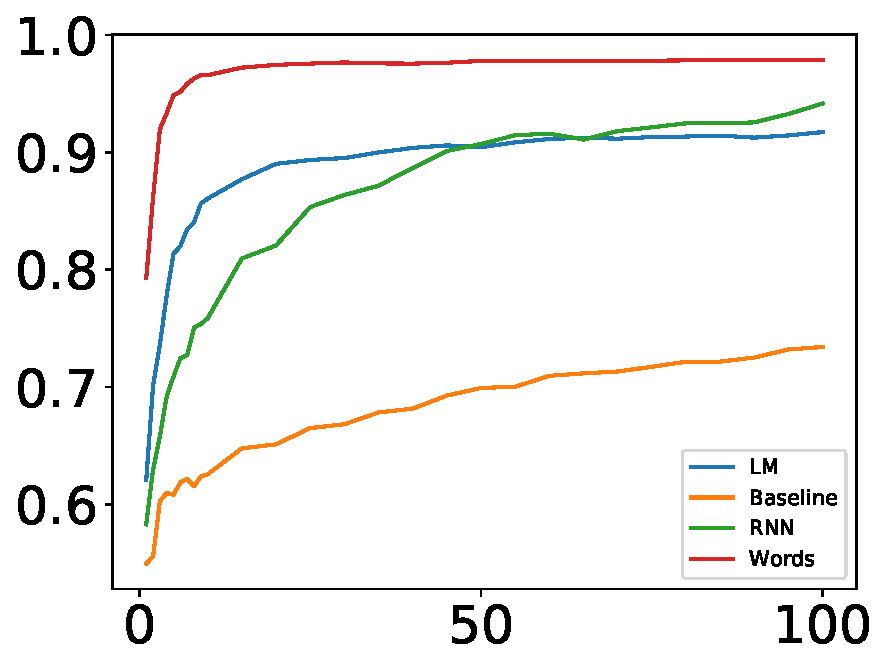
\includegraphics[width=0.48\textwidth]{figures/german_pos_nouns_verbs.pdf}
	\caption{POS accuracy as a function of training examples.}\label{fig:pos-induction}
\end{figure}





\paragraph{Number}
Does the hidden state of the CNLM store an abstract notion of
number?
German nouns can be binned in different classes depending on
the morpheme or morphological process they use to form the plural. We
train a number classifier on a subset of these classes, test on the
others: if model generalizes correctly, it means that it knows about
number independently of its surface expression.

We extracted plural nouns from the German Universal Dependencies treebank \cite{de2006generating,mcdonald2013universal}.
We selected plurals formed with -\emph{n}, -\emph{s}, or -\emph{e} suffixation to train the classifier, and tested on plurals formed with -\emph{r} suffixation or vowel change (\emph{umlaut}).

For the training set, we randomly selected 30 singulars and 30 plurals from each of the training classes.
As plural suffixes make words longer, we used rejection sampling from a single distribution over lengths to ensure that the lengths of the singular and plural examples were approximately matched.
For the test set, we selected all plurals with -\emph{r} suffix or vowel change together with their respective singulars.

As before, we consider an autoencoder and embeddings from a word-level language model as baselines.

To control for the impact of random selection of training samples, we repeated this 200 times and averaged the resulting accuracies on number classification.
Results are summarized in Table \ref{tab:number-results}.


\begin{table}[t]
  \begin{center}
    \begin{tabular}{l|l|l|l}
      &\emph{-n, -s, -e}&\emph{-r}&\emph{Umlaut}\\      \hline
      LSTM& 82.1/68.0/83.7  & \textbf{88.2} & 52.8 \\
      RNN& 77.6/60.0/73.4 & 81.3 & 53.3\\
      Autoencoder& 73.2/54.5/64.4 & 73.8 & 59.2\\
      WordNLM& \textbf{97.1/97.9/98.5} & 86.6 & \textbf{96.7}  \\ % when including OOVs: 81.0/83.8/81.5 & 72.9 & 77.6\\
    \end{tabular}
  \end{center}
  \caption{\label{tab:number-results} Accuracy for classifying number. The random baseline is 50 \%.}
\end{table}

%python char-lm-ud-stationary-separate-bidir-with-spaces-probe-baseline-prediction-wiki-plurals-2-tests-RNN.py  --batchSize 256 --char_dropout_prob 0.01 --char_embedding_size 50 --char_noise_prob 0.0 --hidden_dim 2048 --language german --layer_num 2 --learning_rate 0.1 --nonlinearity tanh --load-from wiki-german-nospaces-bptt-rnn-237671415 --sequence_length 30 --weight_dropout_hidden 0.0 --weight_dropout_in 0.0
%python char-lm-ud-stationary-separate-bidir-with-spaces-probe-baseline-prediction-wiki-plurals-2-tests-words.py  --language german --batchSize 128 --char_embedding_size 200 --hidden_dim 1024 --layer_num 2 --weight_dropout_in 0.1 --weight_dropout_hidden 0.35 --char_dropout_prob 0.0 --char_noise_prob 0.01 --learning_rate 0.2 --load-from wiki-german-nospaces-bptt-words-966024846


The classifier based on word embeddings is overall the most successful, confirming that word embeddings encode number reliably.
Encodings from the CNLM outperform the autoencoder on plurals formed with suffixes, indicating some generalization to unseen plurals beyond orthographic cues.
In the case of -\emph{r} plurals, the CNLM LSTM generalizes better than the word NLM.
In contrast, almost no generalization to plurals formed by vowel change is found, suggesting that the CNLM does not consistently encode noun number in a fully generalizable way -- at least not in a way accessible to a logistic classifier.


\subsection{Capturing syntactic dependencies}
\label{sec:dependencies}

Despite not having pre-defined information about words and morphemes, is the model able to capture non-adjacent syntactic dependencies?
In particular, is it able to do so when dependencies cross one or more words, and thus cannot be reduced to surface n-gram counts?
Note that, for a CNLM, dependencies across even a single word are often already long-distance. % even \emph{``\textbf{la} bell\textbf{a}''} is long distance.
We again focus on German and Italian due to the richness of inflectional morphology in these languages.
Constructions will be language-specific, so we discuss the languages separately. %German and Italian separately (not much in English).

%As usual, specifics of training etc that depart from general setup.




\paragraph{German} We consider 4 constructions:
\begin{inparaenum}[i)]
\item article-noun gender agreement, possibly with material in the middle,
\item determiner-noun case concord, again with material in the middle,
\item preposition case sub-categorization, with material in the middle.
\end{inparaenum}


\paragraph{German Gender Agreement}
Each German noun belongs to one of three genders (masculine, feminine, neuter), which are morphologically marked on the article.
As the article and the noun can be separated by adjectives and adverbs, we can probe not only the CNLM's knowledge of nouns' genders, but also its ability to model gender agreement across distances.
We create stimuli of the form
\begin{enumerate}[label={(\arabic*)}]
	\item \begin{tabular}[t]{lllllll}
	\{\underline{der}, die, das\}& sehr& rote& Baum \\
	article & adverb & adjective & noun \\
	the & very & red & tree
\end{tabular}
\end{enumerate}
where the correct nominative singular article (\emph{der}, in this case) matches the gender of the noun.
We then run the CNLM on the three versions of this phrase (removing whitespace) and record the probabilities it assigns to them.
If it systematically assigns the highest probability to the correct version, we have evidence that the CNLM has learnt the association between the noun and the form of the article.
To indicate that there are word boundaries at the beginning and end of the phrase (e.g., \emph{der} could also be the end of another word), we add a full stop before and after the stimulus when running the CNLM.

%  \cite{de2006generating,mcdonald2013universal}
We select all nominative singular nouns from the German Universal Dependencies treebank. %, and all adjectives from the training set.
We construct four conditions varying the number of adverbs and adjectives between the article and the noun.
We first consider stimuli where no material intervenes.\footnote{Due to syncretism in the article paradigm, there sometimes is ambiguity in the choice of the correct article if the noun's morphology does not uniquely indicate that it is nominative singular. As this affects all feminine nouns, we did not remove such cases. Importantly, this issue is solved as soon as an adjective is present, as their form uniquely indicates that the phrase is nominative singular.}
In the second condition, an adjective with the correct (nominative singular) case ending, randomly selected from the training corpus, is added.
Crucially, the ending of the adjective does not reveal the gender of the noun.
In the third and fourth condition, one (\emph{sehr}) or two adverbs (\emph{sehr extrem}) intervened between the article and the adjective.
These also do not reveal the noun's gender.

Besides the CNLMs and the word-level language model, we also construct an n-gram baseline that chooses the version that occurs most frequently in the training data, and randomly chooses in case of a tie (e.g., if no version was observed).
When running the word-level model, we excluded nouns that were out of vocabulary.

In Figure~\ref{fig:gender}, we report accuracy for nouns from each of the three genders, and the average over the genders.
Across genders and conditions, the word-level LSTM tends to perform best, followed by the CNLM.
While the n-gram baseline performs similarly to the CNLM when there is no intervening material, accuracy drops to the random baseline (0.33) in the presence of an adjective.
%This can partly be attributed to our choice to choose the adjective randomly from the vocabulary.
Note that this would not be mitigated by models that include interpolation with or backoff to lower-order n-grams, as the relevant gender information is present only on the first and last word of each stimulus.
This contrast shows that, while the association between articles and nouns can be learnt from simple corpus statistics, the CNLM has some capability to preserve the relevant information across more than a dozen timesteps.
The RNN CNLM is weaker across conditions, and its accuracy drops to random as more intervening material is present.

The exclusion of OOVs and thus limiting experiments on word-level models to frequent words might create an unfair advantage; running the CNLM only on those stimuli given to the word-level model results in slightly better accuracies but the same pattern of results.

\begin{figure*}
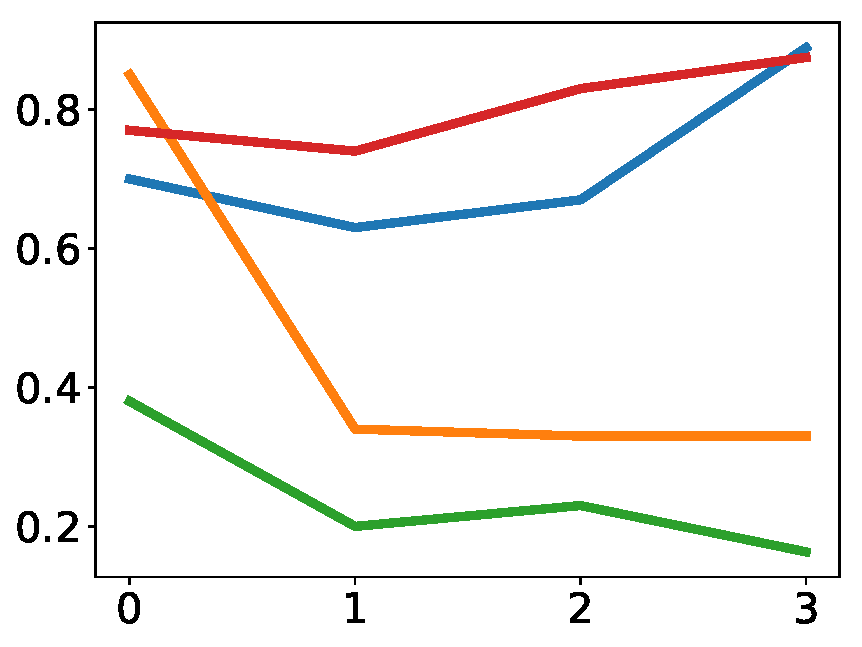
\includegraphics[width=0.24\textwidth]{figures/german-gender-m.pdf}
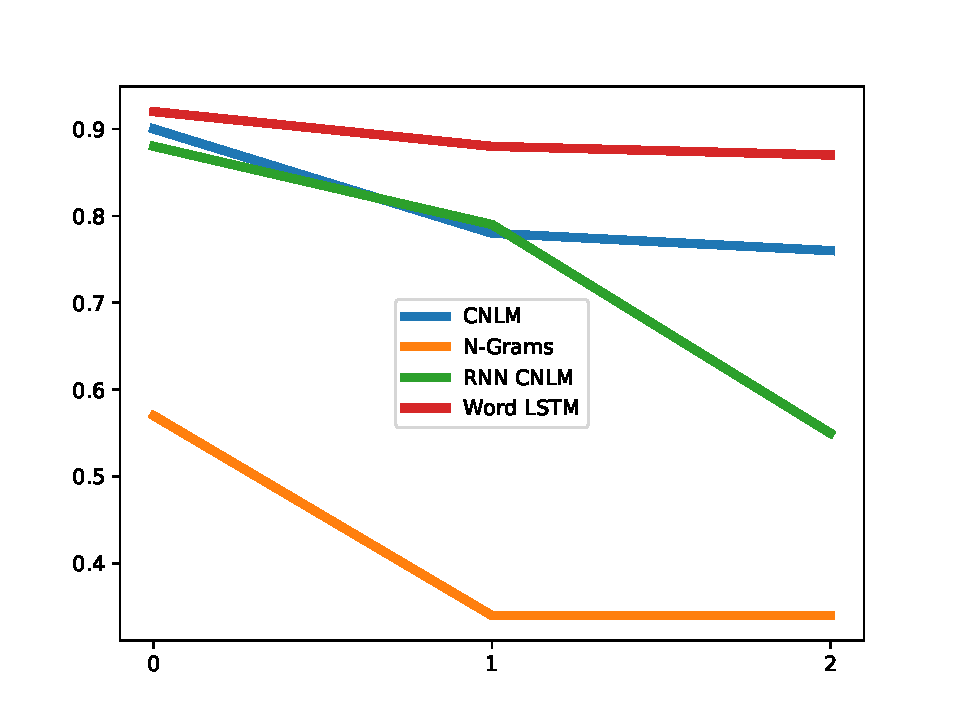
\includegraphics[width=0.24\textwidth]{figures/german-gender-f.pdf}
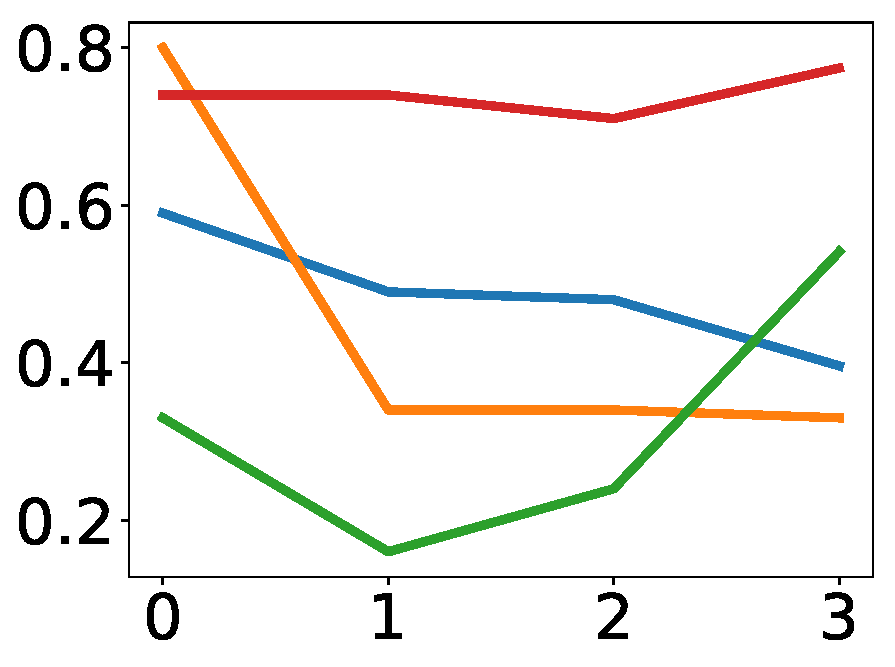
\includegraphics[width=0.24\textwidth]{figures/german-gender-n.pdf}
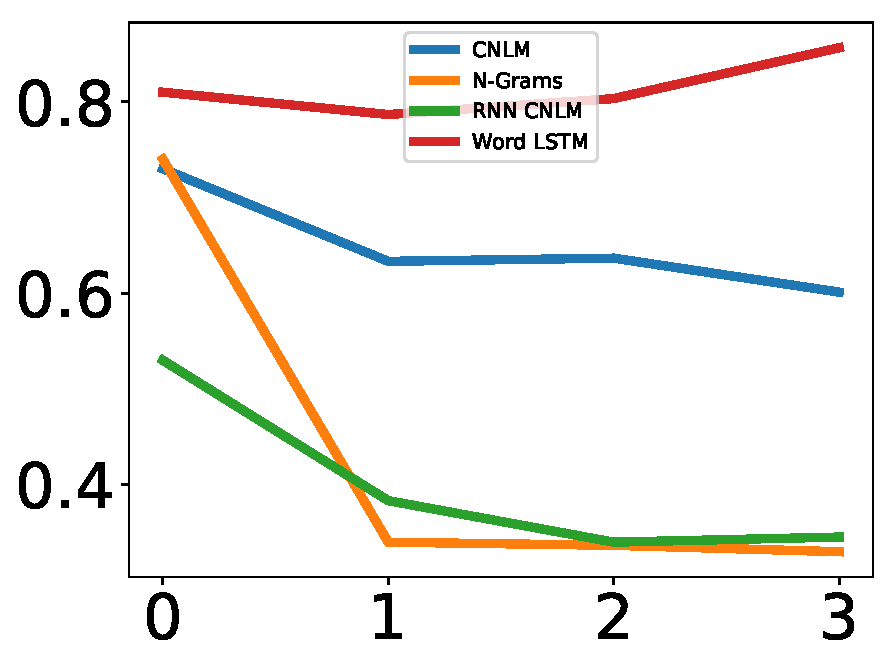
\includegraphics[width=0.24\textwidth]{figures/german-gender-total.pdf}

\centering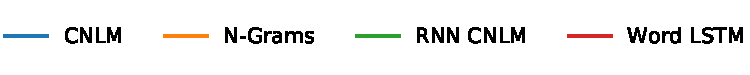
\includegraphics[width=0.5\textwidth]{figures/german-legend.pdf}
\caption{Accuracy on the Gender Agreement task as a function of the number of intervening elements, for masculine, feminine, and neuter nouns, and across all three classes.}\label{fig:gender}
\end{figure*}


\paragraph{Case Agreement}
Here we test the model's knowledge of case agreement between articles and nouns.
We selected the two determiners \emph{dem} and \emph{des}, which unambigously indicate dative and genitive case, respectively, for masculine and neuter nouns.
We also selected all nouns of the appropriate genders that unambigously mark these two cases.
We selected noun lemmas from the Universal Dependencies treebank, and extracted morphological paradigms for Wiktionary to obtain case-marked forms.
We created four conditions, varying the amount of intervening material, as in the gender agreement experiment.

Results are shown in Figure~\ref{fig:case}.
Again, the Word LSTM has the strongest overall performance, but the CNLM is competitive as more elements intervene. Accuracy stays well above 80 \% even as three words intervene.
The n-gram model performs well if there is no intervening material, and at chance otherwise.
Accuracy of the RNN CNLM remains above chance for one or two intervening elements, but drops considerably.

Considering the results for the dative and genitive separately, accuracy slightly increases in the dative case and decreases in the genitive case.
This can be attributed to the higher baseline frequency of dative in German, suggesting that both word- and character-based networks are impacted by unigram frequencies as more words intervene.
This effect is far more pronounced for the RNN CNLM, explaining its overall decrease to chance level.
Again, restricting to words that are in the word-level vocabulary did not change the pattern of results.
\begin{figure}
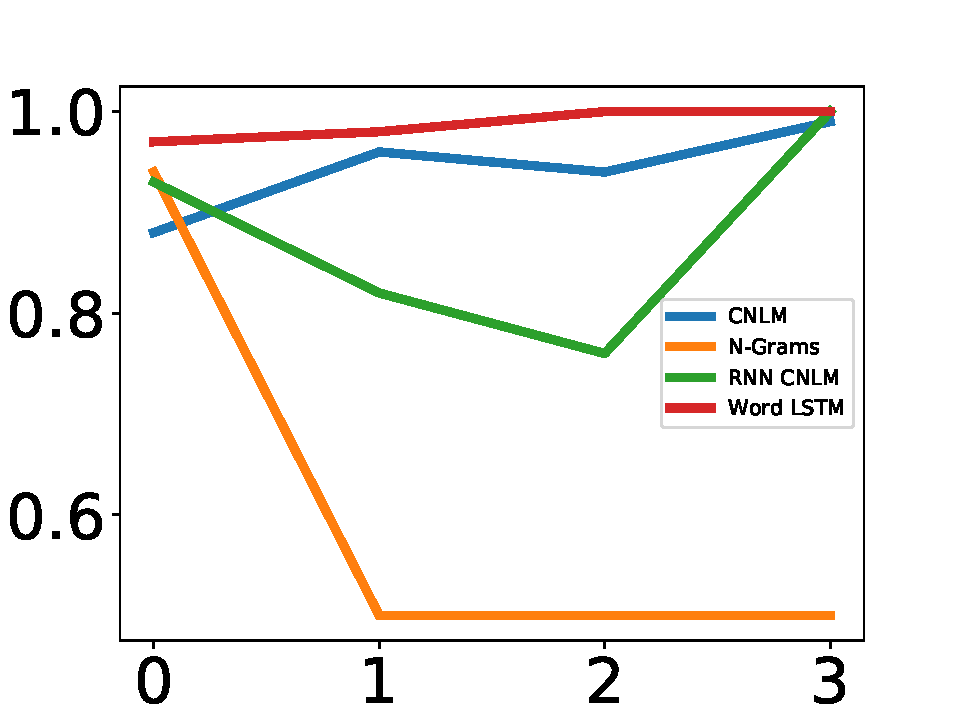
\includegraphics[width=0.23\textwidth]{figures/german-case-Dative.pdf}
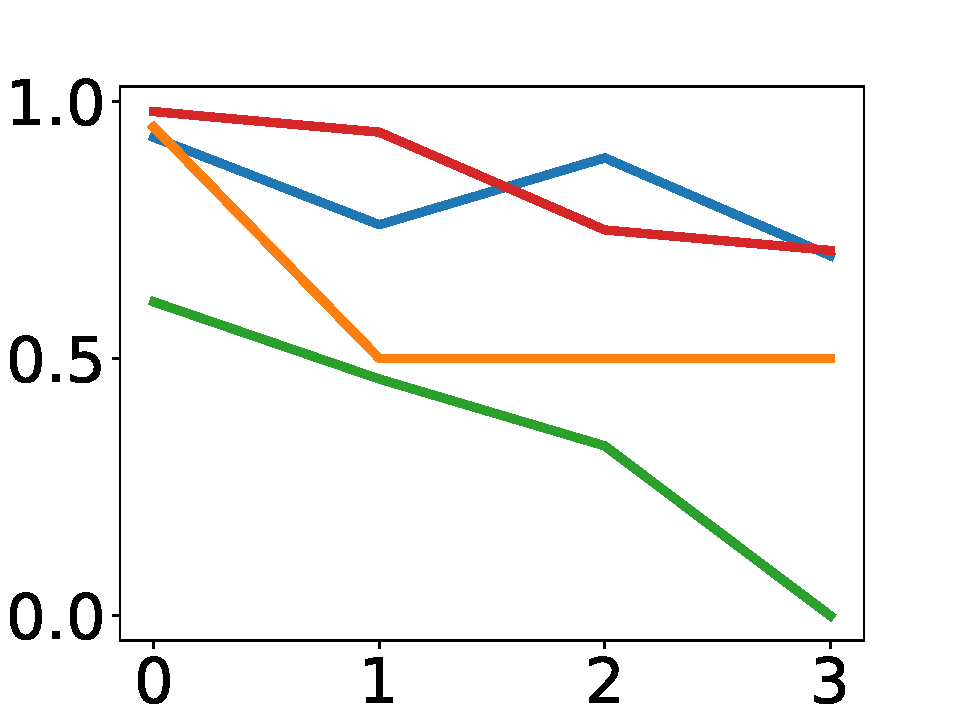
\includegraphics[width=0.23\textwidth]{figures/german-case-Genitive.pdf} \\

\centering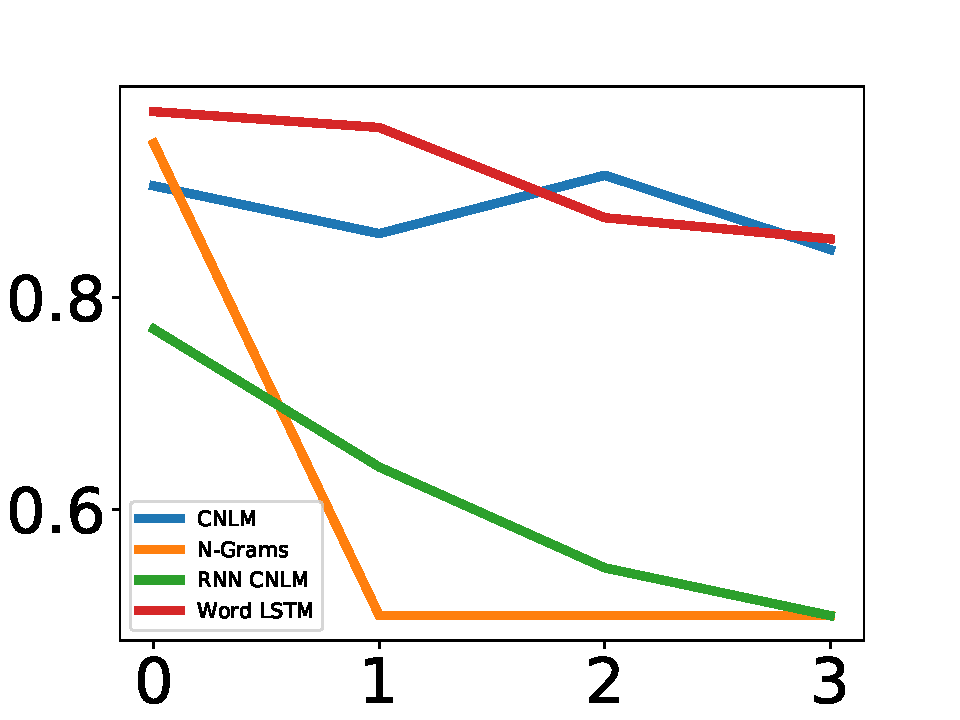
\includegraphics[width=0.24\textwidth]{figures/german-case-total.pdf}

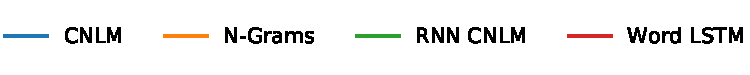
\includegraphics[width=0.5\textwidth]{figures/german-legend.pdf}
	\caption{Accuracy on the Case Agreement task as a function of the number of intervening elements, for dative and genitive phrases (top), and across the two cases (bottom).}\label{fig:case}
\end{figure}

\paragraph{Case Subcategorization}
German verbs and prepositions lexically specify the case appropriate to their objects (mostly dative or accusative).
We probe the CNLM's knowledge of such generalizations using the preposition \textit{mit} `with', which selects for a dative object.

To focus on knowledge of subcategorization (as opposed to inflectional paradigms), we construct objects whose head noun is a nominalized adjective, whose inflection is very regular.
We take all adjectives that occur at least 100 times in the training data, excluding those that end in -\emph{r}, as these often reflected lemmatization problems.

We then selected all sentences containing a `mit' prepositional phrase in the German Universal Dependencies treebank, subject to the constraints that (1) the object is not a pronoun (such objects often are relative or interrogative pronouns and cannot be replaced with a nominal object without sacrificing grammaticality), and (2) the object is a continuous phrase.
For each sentence, we remove the prepositional phrase and replace it by a phrase of the form
\begin{enumerate}[label={(\arabic*)}]
	\item \begin{tabular}[t]{lllllll}
	mit & der & sehr& \{rote, \underline{roten}\} \\
	prep & article  & adverb & adjective \\
	with & the & very  & red one 
\end{tabular}
\end{enumerate}
where only the \emph{-en} version of the adjective is compatible with the case requirement of the preposition.
Note that this correct version is longer than the incorrect one; this ensures that the bias for shorter sequences works against the model.
We construct three conditions by varying the presence and number of adverbs (\emph{sehr} `very', \emph{sehr extrem} `very extremely', \emph{sehr extrem unglaublich} `very extremely incredibly').
As a control for baseline probabilities of the two versions of the adjective, we also created control stimuli where all words up to the preposition were removed, and computed accuracy on these stimuli.
If accuracy is lower on these stimuli than on the full stimuli, we can conclude that baseline probabilities of the two adjective forms cannot explain success on the task.

For the n-gram count model, we only counted the occurrences of the prepositional phrase, omitting the environment.

\begin{figure}
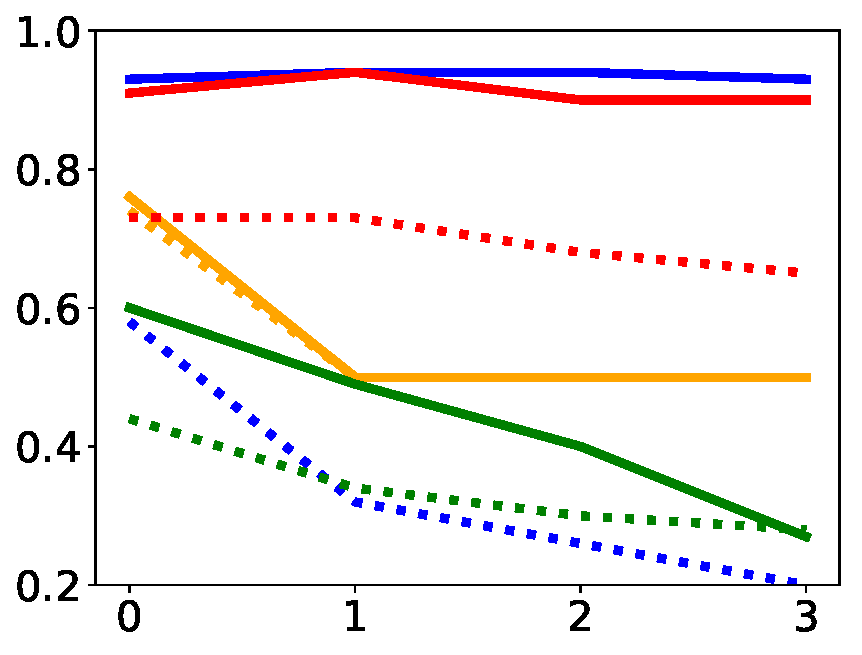
\includegraphics[width=0.48\textwidth]{figures/german-prep-with-control.pdf}

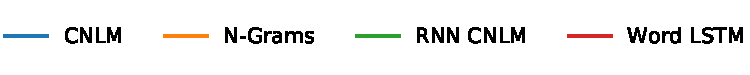
\includegraphics[width=0.48\textwidth]{figures/german-legend.pdf}
\caption{Accuracy on the Subcategorization task as a function of the number of intervening elements. For eavh model, the dashed line indicates accuracy on the control stimuli that do not contain the preposition.}\label{fig:prep}
\end{figure}

Results are shown in Figure~\ref{fig:prep}.
All models except the one based on n-gram counts outperform the accuracy achieved on the control stimuli that did not include the preposition, showing that their performance cannot be attributed to baseline frequencies of the adjective forms, and that they take the preposition into account when choosing the adjective form.
The CNLM slightly outperforms the word-level language model, even though the CNLM has a harder task as it is not limited to the 50,000 most frequent words.
Neither model shows accuracy decay as the number of adverbs increases.
As before, the n-gram model drops to chance as adverbs intervene, while the RNN CNLM starts with low accuracy that decays below chance.



%Results are shown in Table~\ref{tab:ital-agr-results}.
%The word LSTM shows the highest overall performance, closely followed by the LSTM CNLM.
%The RNN performs well on adjective gender, and considerably worse than the CNLM on the other tasks.
%For the CNLMs, the most challenging task was article-noun gender agreement.
%Discussion case-by-case, including how we control for n-gram frequency
%and length.
%Results table with a row for each pattern and a column for each model.


\paragraph{Italian} We consider further constructions from Italian that confirm the results we got in German.
Here, we focus on a  subset of Italian morphology where gender and number are explicitly and systematically
encoded while allowing for tightly controlled comparison of
same-length strings, limited to stimuli unseen in the training corpus.
\begin{inparaenum}[i)]
\item article-noun gender agreement with material in the middle,
\item article-adjective gender agreement, with an adverb in the middle,
\item article-adjective number agreement, with an adverb in the middle.
\end{inparaenum}

\paragraph{Article-Noun Gender Agreement}
%(1) eadj-aonoun:

Similar to German, Italian articles agree with the noun in gender; however, while gender is often unpredictable in German, Italian has a productive system of forming masculine and feminine versions of nouns that differ in the final vowel (-\emph{o} for masculine, -\emph{a} for feminine).
We construct stimuli of the form:
\begin{enumerate}[label={(\arabic*)}]
	\item 
		\begin{tabular}[t]{lllllll}
	a. & \{\underline{il}, la\} & congeniale & candidato \\
   &  the & congenial & candidate (m.) \\
	& \multicolumn{4}{l}{`The congenial male candidate.'} \\
	b. & \{il, \underline{la}\} & congeniale & candidata \\
    &the & congenial & candidate (f.) \\
	& \multicolumn{4}{l}{`The congenial female candidate.'} \\
\end{tabular}
\end{enumerate}

Note that the intervening adjective, ending in -\emph{e}, does not reveal the noun's gender, increasing the distance across which gender information has to be transported.

We constructed these stimuli such that none of the adjective-noun pairs appear in the training data, and all single words appear at least 100 times.
Further, the nouns in -\emph{a} and  -\emph{o} have reasonably balanced frequency (neither form is twice more frequent than the other), or they are both frequent (appear at least 500 times)
As the prenominal adjectives are somewhat marked in Italian, we  we considered only -e adjectives that occur at least with 10 different nouns in the prenominal position.

Results are shown in the first line in Table~\ref{tab:ital-agr-results}.
The word LSTM shows the strongest performance, closely followd by the LSTM CNLM.
Even the RNN CNLM performs strongly above chance.

\paragraph{Article-Adjective Gender Agreement}
We then created an experiment where an adverb intervened between an article and an adjective, both of which were marked for gender:
\begin{enumerate}[label={(\arabic*)}]
	\item 
		\begin{tabular}[t]{lllllll}
	a. & il & meno & \{ \underline{alieno}, aliena \} \\
   &  the & less & alien one  \\
	b. & la & meno & \{ alieno, \underline{aliena} \} \\
    &the & less & alien one \\
\end{tabular}
\end{enumerate}
where we used the adverbs \emph{pi{\`u}} `more', \emph{meno} `less', \emph{tanto} `so much'.
We considered only adjectives that occurred 1K times in the training corpus, as this is the most common kind of adjective in Italian.
We excluded all cases in which the adverb-adjective combination occurred in the training corpus, in either feminine or masculine form.


% /checkpoint/mbaroni/char-rnn-exchange/candidate_adv_aoadj_testset.txt

Results are shown in the second line in Table~\ref{tab:ital-agr-results}; all three models perform almost perfectly.

\begin{table}[t]
  \begin{center}
    \begin{tabular}{l|ll|ll|ll}
	    & \multicolumn{4}{c|}{CNLM} & \multicolumn{2}{c}{\multirow{2}{*}{Word LSTM}}\\
	    &\multicolumn{2}{c|}{\emph{LSTM}}&\multicolumn{2}{c|}{\emph{RNN}} &\\ \hline
% eadj-aonoun
	    Noun Gender & 97&90  & 84&73 & 99&96 \\
%      adv-aoadj
	    Adj. Gender & 99&100 & 100&97 & 98&100 \\
% adv-aeadj
	    Adj. Number & 99&99 & 99&70 & 100&100 \\
    \end{tabular}
  \end{center}
	\caption{\label{tab:ital-agr-results} Results for morphosyntactic tests in Italian. For each model and test, we show accuracy on the two types of stimuli (masculine/feminine for gender, singular/plural for number).}
\end{table}

\paragraph{Article-Adjective Number Agreement}
We then constructed a version of the last test that probed number agreement instead of gender agreement; number marking is similarly very systematic in Italian.
Stimuli had the form
\begin{enumerate}[label={(\arabic*)}]
	\item 
\begin{tabular}[t]{lllllll}
	a. & la & meno & \{ \underline{aliena}, aliene \} \\
   &  the & less & alien one(s)  \\
	b. & le & meno & \{ aliena, \underline{aliene} \} \\
    &the & less & alien one(s) \\
\end{tabular}
\end{enumerate}
% /checkpoint/mbaroni/char-rnn-exchange/candidate_adv_aeadj_testset.txt
Selection of stimuli was  as before, but  we took a 500-occurrences threshold, as feminine plurals are less common.
Further, we manually removed adjectives that did not combine well semantically with the adverbs under consideration (\emph{pi{\`u}, meno, tanto}).

Results are shown in the third line in Table~\ref{tab:ital-agr-results}; the LSTMs perform almost perfectly, while the RNN still performs strongly above chance.






\subsection{Lexical semantics}
\label{sec:semantics}

Finally, we probe the CNLM's knowledge of lexical semantics.
We turn to  English because more resources are available there.

We use the Microsoft Research Sentence Completion task \cite{Zweig:Burges:2011}.
The challenge consists of sentences with a gap, and five words; the model has to choose which word is most appropriate.
The choice is mostly between words of the same syntactic category, and solving the task requires world knowledge for humans to solve; thus this complements the morphosyntactic tests in the previous section.
Language models can be applied to this task by calculing the likelihood of all possible completions of a sentence and selecting the one assigned the highest likelihood.

The domain of the task (Sherlock Holmes novels) is very different from the Wikipedia dataset we are using; thus we addionally trained our models on the training set provided for the task, consisting of 19th century English novels.
We both consider a fresh model trained on that data, and initializing it with the Wikipedia model.
%For comparison, we report results (KN5 from , LSTM from ) from previous work that were trained on the 19th century novels dataset (but the LSTM from that work had Glove embeddings). % \cite{zhang2016top} has a nice table if we want to report more

Results are shown in Figure~\ref{tab:msr-completion-results}.
The models trained on Wikipedia perform poorly but above chance, reflecting the domain mismatch.
When trained on data from the appropriate domain, the LSTM CNLM outperforms many previously reported results from word-level neural models. %, and approaches the best published results.
%, held by approaches developed for the completion task \cite{woods2016exploiting}.
% The best results I could find, https://github.com/ctr4si/sentence-completion, are much better than the best peer-reviewed published ones
The vanilla RNN is not successful even when trained on the in-domain data, contrasting with \emph{word}-based vanilla RNNs, whose performance, while below that of LSTMs, is much stronger.

This experiment shows that a CNLM, trained without word boundaries, learns lexical knowledge to a degree competitive with models trained on words.

\begin{table}[t]
  \begin{center}
    \begin{tabular}{l|l|l|l|llllll}
      \multicolumn{1}{c}{}& Model \\
LSTM CNLM	    &      34.1/59.0/59.2 \\
	    RNN CNLM &     24.3/24.0/27.1 \\
	    Word LSTM & 37.1/.../... \\ \hline
	    Random & 20 \\
	    KN5   & 40.0 \\
            Word RNN & 45.0 \\
	    Word LSTM  & 55.96 \\
Skipgram + RNNs  & 58.9 \\
LdTreeLSTM  & 60.67 \\
            \citet{woods2016exploiting} &  61.44 \\
\citet{melamud2016context2vec} & 65.1 \\
    \end{tabular}
  \end{center}
  \caption{\label{tab:msr-completion-results} Results on MSR Sentence Completion. KN5 is from \cite{Mikolov:2012}, Word LSTM and LdTreeLSTM are from\cite{zhang2016top}, Skipgram+RNNs from \cite{Mikolov:etal:2013b}.}
\end{table}






\section{Discussion}
\label{sec:discussion}

We probed the linguistic information induced by an LSTM language model
trained on unsegmented text at the character level. We found that the
model stores implicit knowledge about phonotactic constraints, word
units, major morphosyntactic classes, non-adjacent syntactic agreement
and subcategorization phenomena and even some degree of semantic
knowledge. While a more standard model pre-initialized with a word
vocabulary and reading tokenized input was in general superior on the
higher-level tasks, the performance of our agnostic model did not
generally lag much behind, suggesting that the word bias is helpful
but not fundamental. The performance of character-level RNN was
considerably less consistent than that of the equivalent LSTM, suggesting that
the ability of the latter to track information across longer time
steps is important to extract linguistic generalizations from the raw
input. Importantly, n-gram baselines only relying on adjacent string
statistics fail almost all tests, showing that the neural models
are tapping into somewhat deeper linguistic templates.

Our results are very preliminary in many ways. The tests we used are
generally simple \cite[we did not attempt, for example, to model
long-distance subject-verb agreement, a task that is challenging even
for word-based models:][]{Linzen:etal:2016}, and they only probe a
small subset of linguistic rules. Still, they do suggest that a large
corpus, combined with the very weak priors encoded in an LSTM, might
suffice to discover generalizations that appear to be of a genuine
linguistic nature. It is entirely plausible, of course, that much
stronger priors would be needed when using smaller amounts of training
data, an hypothesis that we would like to study in future work.

One aspect that we find particularly intriguing is that, unlike the
standard word-based models, our CNLMs do not have a morpheme- or
word-based lexicon. Any information the network might acquire about
units larger than characters must be stored in its recurrent
weights. Given that nearly all contemporary linguistics recognizes a
central role to the lexicon \cite[see, e.g.,][for different
perspectives]{Sag:etal:2003,Goldberg:2005,Radford:2006,Bresnan:etal:2016,Jezek:2016},
in future work we would like to explore how lexical knowledge is
implicitly encoded in the distributed memory of our CNLMs.

One of our original motivations for not assuming word primitives is that a rigid word notion is problematic both cross-linguistically (cf.~polysynthetic and agglutinative languages) and when analyzing a single language (cf.~the common  view  that the lexicon hosts units at different levels of the linguistic hierarchy, from  morphemes to large syntactic constructions). Our brief analysis of the CNLM over- and undersegmentations suggested that it is indeed capable to flexibly store information about units at different levels. However, this topic  remained largely unexplored, and we plan to systematically tackle it in future work.



\bibliography{marco,michael}
\bibliographystyle{acl_natbib}

\end{document}


